% Options for packages loaded elsewhere
\PassOptionsToPackage{unicode}{hyperref}
\PassOptionsToPackage{hyphens}{url}
%
\documentclass[
  ignorenonframetext,
]{beamer}
\usepackage{pgfpages}
\setbeamertemplate{caption}[numbered]
\setbeamertemplate{caption label separator}{: }
\setbeamercolor{caption name}{fg=normal text.fg}
\beamertemplatenavigationsymbolsempty
% Prevent slide breaks in the middle of a paragraph
\widowpenalties 1 10000
\raggedbottom
\setbeamertemplate{part page}{
  \centering
  \begin{beamercolorbox}[sep=16pt,center]{part title}
    \usebeamerfont{part title}\insertpart\par
  \end{beamercolorbox}
}
\setbeamertemplate{section page}{
  \centering
  \begin{beamercolorbox}[sep=12pt,center]{part title}
    \usebeamerfont{section title}\insertsection\par
  \end{beamercolorbox}
}
\setbeamertemplate{subsection page}{
  \centering
  \begin{beamercolorbox}[sep=8pt,center]{part title}
    \usebeamerfont{subsection title}\insertsubsection\par
  \end{beamercolorbox}
}
\AtBeginPart{
  \frame{\partpage}
}
\AtBeginSection{
  \ifbibliography
  \else
    \frame{\sectionpage}
  \fi
}
\AtBeginSubsection{
  \frame{\subsectionpage}
}
\usepackage{amsmath,amssymb}
\usepackage{lmodern}
\usepackage{iftex}
\ifPDFTeX
  \usepackage[T1]{fontenc}
  \usepackage[utf8]{inputenc}
  \usepackage{textcomp} % provide euro and other symbols
\else % if luatex or xetex
  \usepackage{unicode-math}
  \defaultfontfeatures{Scale=MatchLowercase}
  \defaultfontfeatures[\rmfamily]{Ligatures=TeX,Scale=1}
\fi
\usetheme[]{Madrid}
\usecolortheme{beaver}
% Use upquote if available, for straight quotes in verbatim environments
\IfFileExists{upquote.sty}{\usepackage{upquote}}{}
\IfFileExists{microtype.sty}{% use microtype if available
  \usepackage[]{microtype}
  \UseMicrotypeSet[protrusion]{basicmath} % disable protrusion for tt fonts
}{}
\makeatletter
\@ifundefined{KOMAClassName}{% if non-KOMA class
  \IfFileExists{parskip.sty}{%
    \usepackage{parskip}
  }{% else
    \setlength{\parindent}{0pt}
    \setlength{\parskip}{6pt plus 2pt minus 1pt}}
}{% if KOMA class
  \KOMAoptions{parskip=half}}
\makeatother
\usepackage{xcolor}
\IfFileExists{xurl.sty}{\usepackage{xurl}}{} % add URL line breaks if available
\IfFileExists{bookmark.sty}{\usepackage{bookmark}}{\usepackage{hyperref}}
\hypersetup{
  pdftitle={LDA主题模型},
  pdfauthor={苏烨},
  hidelinks,
  pdfcreator={LaTeX via pandoc}}
\urlstyle{same} % disable monospaced font for URLs
\newif\ifbibliography
\usepackage{longtable,booktabs,array}
\usepackage{calc} % for calculating minipage widths
\usepackage{caption}
% Make caption package work with longtable
\makeatletter
\def\fnum@table{\tablename~\thetable}
\makeatother
\usepackage{graphicx}
\makeatletter
\def\maxwidth{\ifdim\Gin@nat@width>\linewidth\linewidth\else\Gin@nat@width\fi}
\def\maxheight{\ifdim\Gin@nat@height>\textheight\textheight\else\Gin@nat@height\fi}
\makeatother
% Scale images if necessary, so that they will not overflow the page
% margins by default, and it is still possible to overwrite the defaults
% using explicit options in \includegraphics[width, height, ...]{}
\setkeys{Gin}{width=\maxwidth,height=\maxheight,keepaspectratio}
% Set default figure placement to htbp
\makeatletter
\def\fps@figure{htbp}
\makeatother
\setlength{\emergencystretch}{3em} % prevent overfull lines
\providecommand{\tightlist}{%
  \setlength{\itemsep}{0pt}\setlength{\parskip}{0pt}}
\setcounter{secnumdepth}{5}
\usepackage[UTF8, heading = false, scheme = plain]{ctex}



\newfontfamily\WRYaHei{微软雅黑}%新建微软雅黑字体,注意,使用\newfontfamily命令创建的字体只能用于英文。是吗?是的,fontspec宏包提供了\fontspec、\setmainfont、\setsansfont、\setmonofont、\newfontfamily命令,当使用ctex宏包的时候,这些命令只对英文和阿拉伯数字有效。而ctex所使用的xeCJK宏包里所提供的\setCJKmainfont、\setCJKsansfont、\setCJKmonofont、\setCJKmonofont、\setCJKmonofont、\setCJKfamilyfont、\setCJKfallbackfamilyfont则只对CJK字体有效。
\setCJKfamilyfont{WRYaHei}{微软雅黑}%新建微软雅黑字体,注意,使用\setCJKfamilyfont命令创建的字体只能用于中文。
\newcommand{\WRYaHeiZH}{\WRYaHei\CJKfamily{WRYaHei}}%新建一个命令,对中文和英文都使用微软雅黑
\setCJKmainfont{微软雅黑}
\setsansfont{Times New Roman}%这个是用来设置正文中的英语使用Times New Roman的,(可是为什么是这一个而不是另外的两个呢?)

%常规大小
\renewcommand{\normalsize}{\fontsize{12}{12}\selectfont}%把常规大小设置为12pt
%标题字体
\setbeamerfont{title}{family=\WRYaHeiZH,size=\fontsize{28}{28}\selectfont,series=\bfseries}%设置标题的字体为微软雅黑,加粗,字号为28pt
\setbeamerfont{subtitle}{family=\WRYaHeiZH,size=\fontsize{14}{14}\selectfont,series=\bfseries}%设置标题的字体为微软雅黑,加粗,字号为28pt


%机构字体
\setbeamerfont{institute}{family=\songti,size=\fontsize{12}{12}\selectfont,series=\bfseries}%设置机构的字体为宋体,加粗,字号为12pt
%作者字体
\setbeamerfont{author}{parent=institute}%设置作者的字体和机构的字体相同
%日期字体
\setbeamerfont{date}{parent=institute}%设置日期的字体和机构的字体相同
%list元素的字体
\setbeamerfont{item projected}{size=\fontsize{12}{12}\selectfont,series=\mdseries}
\setbeamerfont{itemize/enumerate subbody}{family=\kaishu,size=\fontsize{12}{12}\selectfont,series=\mdseries}

%帧标题字体
\setbeamerfont{frametitle}{family=\WRYaHeiZH,size=\fontsize{18}{18}\selectfont,series=\bfseries}%设置帧标题的字体为微软雅黑,加粗,字号为18pt
%帧子标题字体
\setbeamerfont{framesubtitle}{family=\kaishu,size=\fontsize{14}{14}\selectfont,series=\bfseries}%设置帧标题的字体为微软雅黑,加粗,字号为14pt

%页眉字体
%\setbeamerfont{headline}{size=\fontsize{12}{12}\selectfont}%设置页眉的字号为16pt,没有办法呀,如果按照经验丰富的老专家的要求使用24pt的话,这里还是太丑了,我最大能接受的就是16pt了。如果这不行,那么只能不要页眉了

%页脚字体
\setbeamerfont{footline}{size=\fontsize{8}{8}\selectfont}%设置页脚的字体等于页眉字体
%盒子环境
%标题字体
\setbeamerfont{block title}{size=\fontsize{14}{14}\selectfont,series=\bfseries}%设置盒子环境的标题的字体为微软雅黑,加粗,字号为14pt


%%%%%%%%%%%%%%%%%%%%%%%%%%%%% 题注  %%%%%%%%%%%%%%%%%%%%%%%%%%%
\setbeamertemplate{caption}[numbered]
%\setbeamerfont{caption}{size=\scriptsize}
\setbeamerfont{caption}{size=\fontsize{10}{10}\selectfont}
\renewcommand\figurename{图}
\renewcommand\tablename{表}
%%%%%%%%%%%%%%%%%%%%%%%%%%%%%%%%%%%%%%%%%%%%%%%%%%%%%%%%%%%%%%%%



%%%%%%%%%%%%%%%%%%%%%%%%%%%    footline     %%%%%%%%%%%%%%%%%%%%%%%%%%%%%
\defbeamertemplate{footline}{NGEGFootlineTemplate}{%
	\leavevmode% 离开vmode,也就是离开竖直模式,进入水平模式
	\hbox{%
%		\begin{beamercolorbox}[wd=.3\paperwidth,ht=2.25ex,dp=1ex,center]{author in head/foot}%
%			\ifnum \the\value{page}>1 \usebeamerfont{author in head/foot}\insertshortauthor\fi
%		\end{beamercolorbox}%
%		\begin{beamercolorbox}[wd=.4\paperwidth,ht=2.25ex,dp=1ex,center]{title in head/foot}%
%			\ifnum \the\value{page}>1 \usebeamerfont{title in head/foot}\insertshorttitle\fi
%		\end{beamercolorbox}%
%		\begin{beamercolorbox}[wd=0.3\paperwidth,ht=2.25ex,dp=1ex,center]{date in head/foot}%
%			\ifnum \the\value{page}>1 \insertframenumber{} / \inserttotalframenumber\fi
%	\end{beamercolorbox}}%
%	\vskip0pt%
	\begin{beamercolorbox}[wd=.25\paperwidth,ht=2.25ex,dp=1ex,center]{author in head/foot}%
    \usebeamerfont{author in head/foot}\insertshortauthor
  	\end{beamercolorbox}%
  	\begin{beamercolorbox}[wd=.25\paperwidth,ht=2.25ex,dp=1ex,center]{title in head/foot}%
    \usebeamerfont{author in head/foot}\insertshortdate
  	\end{beamercolorbox}%
  	\begin{beamercolorbox}[wd=.4\paperwidth,ht=2.25ex,dp=1ex,center]{author in head/foot}%
    \usebeamerfont{title in head/foot}\insertshorttitle
  	\end{beamercolorbox}%
  	\begin{beamercolorbox}[wd=0.1\paperwidth,ht=2.25ex,dp=1ex,right]{title in head/foot}%
    \insertframenumber{} / \inserttotalframenumber\hspace*{2ex}
  	\end{beamercolorbox}}%
  	\vskip0pt%
}

\setbeamertemplate{footline}[NGEGFootlineTemplate]
%%%%%%%%%%%%%%%%%%%%%%%%%%%%%%%%%%%%%%%%%%%%%%%%%%%%%%%%%%%%%%%%%%%%%%%%%%%%%%%%%

% \RequirePackage{bbding}
% %\RequirePackage{arev}
% \newlength{\HeightOfItem}
% \newlength{\HeightOfSubItem}
% \settoheight{\HeightOfItem}{\usebeamerfont*{itemize/enumerate body}{item元素字体高度}}
% \settoheight{\HeightOfSubItem}{\usebeamerfont*{itemize/enumerate subbody}{subitem元素字体高度}}
% \setbeamercolor{structure}{fg=red,bg=white!90!gray}
% \defbeamertemplate{itemize item}{NGEGItemizeItemTemplate}
% 	{
% 		\raisebox{-0.2\HeightOfItem}{\PencilRightUp}
% 	}
% \setbeamertemplate{itemize item}[NGEGItemizeItemTemplate]
% 
% \defbeamertemplate{itemize subitem}{NGEGItemizeSubitemTemplate}
% 	{
% 		\raisebox{-0.2\HeightOfSubItem}{\HandRight}
% 	}
% \setbeamertemplate{itemize subitem}[NGEGItemizeSubitemTemplate]
% 
% 
% \defbeamertemplate{enumerate item}{NGEGEnumerateItemTemplate}
% 	{
% 		\usebeamercolor[structure]{item projected}
% 		\raisebox{-0.5\HeightOfItem}{\checkmark}
% 	}
% \setbeamertemplate{enumerate item}[NGEGEnumerateItemTemplate]

% 无序列表形状
\setbeamertemplate{itemize items}[triangle]
% 有序列表
\setbeamertemplate{enumerate items}[default]

\setbeamercolor{itemize item}{fg=red}
% 可以肯定的是,目录中的标题编号也使用了enumerate环境。故下面两个fg必须保持一致,不然修改不成功。
\setbeamercolor{enumerate item}{fg=red}
\setbeamercolor{section number projected}{fg=red,bg=white!90!gray}
\ifLuaTeX
  \usepackage{selnolig}  % disable illegal ligatures
\fi

\title{LDA主题模型}
\subtitle{原理详解与代码实战}
\author{苏烨}
\date{2021-12-15}
\institute{统计与数学学院}

\begin{document}
\frame{\titlepage}

\begin{frame}[allowframebreaks]
  \tableofcontents[hideallsubsections]
\end{frame}
\hypertarget{ux5199ux5728ux524dux9762}{%
\section{写在前面}\label{ux5199ux5728ux524dux9762}}

\begin{frame}{写在前面}
\(\quad\)在机器学习领域,关于LDA有两种含义,一是「线性判别分析(Linear Discriminant Analysis)」,是一种经典的降维学习方法;一是我们要讲的「隐含狄利克雷分布(Latent Dirichlet Allocation)」,是一种概率主题模型,主要用来文本分类,在NLP领域有重要应用。

\(\quad\)LDA主题模型,在PLSA模型的基础上引入了参数的先验分布的概念,能够对文本信息进行语义抽取,为各领域科研人员提供了文本主题挖掘的新途径。目前它已经被广泛应用于文本信息检索、话题检测和跟踪、线上消费者偏好特征研究、错误报告诊断等诸多领域,产生了许多研究成果。
\end{frame}

\hypertarget{ldaux6a21ux578bux7684ux4ee3ux7801ux5b9eux73b0}{%
\section{LDA模型的代码实现}\label{ldaux6a21ux578bux7684ux4ee3ux7801ux5b9eux73b0}}

\begin{frame}{目前,我在网上找到的实现方式主要有以下3种(都先用jieba将词分好):}
\protect\hypertarget{ux76eeux524dux6211ux5728ux7f51ux4e0aux627eux5230ux7684ux5b9eux73b0ux65b9ux5f0fux4e3bux8981ux6709ux4ee5ux4e0b3ux79cdux90fdux5148ux7528jiebaux5c06ux8bcdux5206ux597d}{}
\begin{enumerate}[<+->]
\tightlist
\item
  使用gensim(Python)里的doc2bow向量化,然后用ldamodel
\item
  使用sklearn(Python)里的CountVectorizer向量化,然后用LatentDirichletAllocation建模
\item
  R语言lda包进行模型训练,使用LDAvis进行可视化。
\end{enumerate}

(图\ref{fig:fig1})
\end{frame}

\begin{frame}{LDAvis可视化demo}
\protect\hypertarget{ldavisux53efux89c6ux5316demo}{}
\begin{figure}

{\centering 
\includegraphics[width=0.5\linewidth,height=0.5\textheight]{pic/LDAdemo} 

}

\caption{作图样例}\label{fig:fig1}
\end{figure}
\end{frame}

\hypertarget{ldaux7684ux6570ux5b66ux539fux7406}{%
\section{LDA的数学原理}\label{ldaux7684ux6570ux5b66ux539fux7406}}

\hypertarget{plsa}{%
\subsection{pLSA}\label{plsa}}

\begin{frame}{pLSA}
\(\quad\)LDA是一种典型的词袋模型,它的基本假设是一篇文档是由一组词构成的一个集合,词与词之间没有顺序以及先后关系。一篇文档可以包含多个主题,文档中每一个词都由其中的一个主题生成。

\(\quad\)经典LDA主题模型的三层贝叶斯模型:
\end{frame}

\begin{frame}{LDA模型}
\protect\hypertarget{ldaux6a21ux578b}{}
\begin{figure}
\centering

\includegraphics{./pic/Smoothed_LDA.jpg}
\caption{Smoothed\_LDA}
\end{figure}
\end{frame}

\begin{frame}{LDA模型}
\protect\hypertarget{ldaux6a21ux578b-1}{}
\(\quad\)如上图所示,在LDA模型中一篇文档生成的方式如下:

\begin{itemize}
\item
  从狄利克雷分布\(\alpha\)中取样生成文档\(i\)的主题分布\(\theta_i\)
\item
  从主题的多项式分布\(\theta_i\)中取样生成文档\(i\)第\(j\)个词\(w_{i,j}\)的主题\(z_{i,j}\)
\item
  从狄利克雷分布\(\beta\)中取样生成主题\(z_{i,j}\)的词语分布\(\phi_{z_{i,j}}\)
\item
  从词语的多项式分布\(\phi_{z_{i,j}}\)中采样最终生成词语\(w_{i,j}\)
\end{itemize}

\(\quad\)LDA主题建模的过程,概括来说就是通过给定的训练文本集学习出参数\(\alpha\)和\(\beta\)。而参数\(\alpha\)和\(\beta\)的估计,可以由EM推断和Gibbs采样算法得到。
\end{frame}

\hypertarget{ux5bf9ux6bd4}{%
\subsection{对比}\label{ux5bf9ux6bd4}}

\begin{frame}{对比}
\begin{columns}[T]
\begin{column}{0.48\textwidth}
My topic for this slide

\scalebox{0.35}{
%latex.default(head(mtcars), file = "", table.env = FALSE, center = "none")%
\begin{tabular}{lrrrrrrrrrrr}
\hline\hline
\multicolumn{1}{l}{head}&\multicolumn{1}{c}{mpg}&\multicolumn{1}{c}{cyl}&\multicolumn{1}{c}{disp}&\multicolumn{1}{c}{hp}&\multicolumn{1}{c}{drat}&\multicolumn{1}{c}{wt}&\multicolumn{1}{c}{qsec}&\multicolumn{1}{c}{vs}&\multicolumn{1}{c}{am}&\multicolumn{1}{c}{gear}&\multicolumn{1}{c}{carb}\tabularnewline
\hline
Mazda RX4&$21.0$&$6$&$160$&$110$&$3.90$&$2.620$&$16.46$&$0$&$1$&$4$&$4$\tabularnewline
Mazda RX4 Wag&$21.0$&$6$&$160$&$110$&$3.90$&$2.875$&$17.02$&$0$&$1$&$4$&$4$\tabularnewline
Datsun 710&$22.8$&$4$&$108$&$ 93$&$3.85$&$2.320$&$18.61$&$1$&$1$&$4$&$1$\tabularnewline
Hornet 4 Drive&$21.4$&$6$&$258$&$110$&$3.08$&$3.215$&$19.44$&$1$&$0$&$3$&$1$\tabularnewline
Hornet Sportabout&$18.7$&$8$&$360$&$175$&$3.15$&$3.440$&$17.02$&$0$&$0$&$3$&$2$\tabularnewline
Valiant&$18.1$&$6$&$225$&$105$&$2.76$&$3.460$&$20.22$&$1$&$0$&$3$&$1$\tabularnewline
\hline
\end{tabular}
}

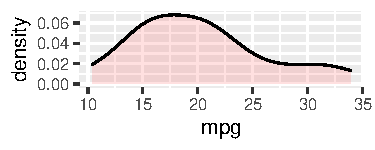
\includegraphics{LDApre_files/figure-beamer/unnamed-chunk-1-1.pdf}
\end{column}

\begin{column}{0.48\textwidth}
\begin{itemize}
\tightlist
\item
  Here is some Bullet Text
\item
  And some more

  \begin{itemize}
  \tightlist
  \item
    Subtext
  \item
    More Subtext
  \end{itemize}
\end{itemize}
\end{column}
\end{columns}
\end{frame}

\end{document}
